Da bei der Messung des EOGs die Daten direkt vom Mikrocontroller zu einem Server geschickt werden und dort auf einer Datenbank gespeichert werden, m�ssen diese zur Ansicht der Daten in der App zuerst vom Server angefragt werden. Wenn in der App zur Datenansicht gewechselt wird, entweder vom Loginfenster oder von der Weckeransicht, wird von einem Widget eine Funktion aufgerufen, in der ein Post-Request an den Server gestellt wird. Der body dieses Requests enth�lt die momentan g�ltige User-ID. Am Server werden alle Daten, die zu dieser ID vorhanden sind gesammelt und ebenfalls in einem Post-Request im JSON-Format zur�ckgesendet. Diese Daten werden dann in der App weiter verwertet. Im Folgenden werden alle einzelnen Schritte n�her erl�utert. 

\paragraph{Async functions} \label{MADataFetching_AsyncFunctions}

Da Vorg�nge wie das Warten auf eine Antwort des Servers nach dem Senden eines POST-Requests lange dauern, w�re es nicht gut, wenn alle anderen Vorg�nge w�hrenddessen blockiert sind. Deshalb gibt es Unterscheidungen zwischen synchronen und asynchronen Vorg�ngen. Bei synchronen Operationen wird ein Schritt nach dem anderen abgehandelt, w�hrend bei asynchronen Operationen w�hrenddessen andere Operationen durchgef�hrt werden k�nnen. Die Klasse, die f�r asynchrone Vorg�nge im Flutter-Framework verwendet wird ist die Future\flq T\frq{} Klasse. Ein \glqq future\grqq{} ist eine Instanz der Klasse Future und ist das Ergebniss einer asynchronen Funktion. Wenn nun eine asynchrone Funktion aufgerufen wird, wird ein unvollst�ndeiges future zur�ckgegeben. Dieses future wartet auf den wirklichen Wert, der von der Funktion zur�ckgegeben wird (falls eine Funktion einen R�ckgabewert hat). \\
Dies sorgt daf�r, dass w�hrend auf die Antwort des Servers gewartet werden muss, alle anderen Vorg�nge in der App weiter bestehen bleiben.

\paragraph{HTTP Requests} \label{}

Es gibt eine Reihe von Requests, die im HTTP-Protokoll angef�hrt sind und oft in zur Datenvermittelung verwendet werden. Zwei der h�ufigsten davon sind der POST- und der GET-Request. Diese beiden unterscheiden sich in mehreren Hinsichten. Wie der Name es annehmen l�sst ist ein GET-Request urspr�nglich f�r die Anfrage an einen Server nach Daten und ein POST-Request f�r das Vermitteln von Daten an den Server gedacht. Dies muss in der Praxis allerdings nicht immer eingehalten werden\cite{reg413}. \\
Einer der wichtigsten Unterschiede ist, dass bei einem GET-Request die gesamte Anfrage im Header eines Requests angef�hrt ist, und somit die L�nge auch an die maximale URL-L�nge eines Browsers angepasst werden muss; Ein GET-Request kann also f�r Internet Explorer zum Beispiel maximal 2.048 Zeichen, abz�glich der Anzahl der Zeichen des Pfads, betragen. \\
Bei einem POST-Request ist das nicht der Fall, da der Inhalt eines POST-Requests nicht im header, sondern im Message-body angef�hrt wird\cite{reg413},\cite{reg414}. \\

\paragraph {Implementierung} \label{MADataFetching_Implementierung}

\begin{figure}[H]
	\centering
		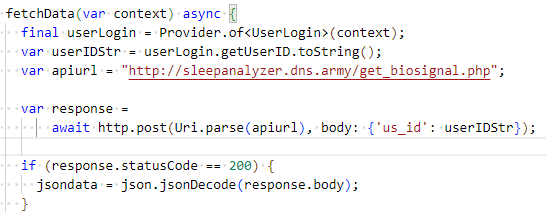
\includegraphics[width=0.9\textwidth]{Gartner/assets/async_post_json.png}
	\caption{Quellcodeausschnitt zur Kommunikation mit dem Server}
	\label{fig:async_post_json}
\end{figure}

In Abbildung \ref{fig:async_post_json} ist die Funktion zur Anfrage und Erhaltung der Daten vom Server zu sehen. Zuerst wird ein POST-Request geschickt, in dessen body die Benutzer-ID festgelegt ist. Die Antwort des Servers erfolgt im JSON-Format und muss dekodiert werden. 

